\usepackage{xcolor}
\usepackage{afterpage}
\usepackage{pifont,mdframed}
\usepackage[bottom]{footmisc}
\usepackage{caption}


\createsection{\Grader}{Sample grader}
\createsection{\Specs}{Specifiche}
\createsection{\Visualizzatore}{Visualizzatore}

\renewcommand{\inputfile}{\texttt{stdin}}
\renewcommand{\outputfile}{\texttt{stdout}}
\makeatletter
\renewcommand{\this@inputfilename}{\texttt{stdin}}
\renewcommand{\this@outputfilename}{\texttt{stdout}}
\makeatother

% % % % % % % % % % % % % % % % % % % % % % % % % % % % % % % % % % % % % % % % % % %
% % % % % % % % % % % % % % % % % % % % % % % % % % % % % % % % % % % % % % % % % % %

In occasion of the XIX edition of the Italian Olympics in Informatics, the
council of Matera decided to build $N$ skyscrapers, each of them assigned to a
different builder. The height of each skyscraper is set by Monica, as the
supreme authority in the Olympiads, with the goal of building the highest
possible skyscrapers while keeping everyone happy.

According to the budget of the $i$-th builder, the $i$-th skyscraper can be
built up to a maximum height of $H[i]$. Moreover, some builders are worried of
looking bad when compared to their competitors, so they decided to set limits to
how much the other skyscraper can ``surpass'' theirs.

The builders set $M$ constraints. Each constraint $j$ is given as three numbers
$A_j$, $B_j$, $C_j$ and specifies that the owner of the $A_j$-th skyscraper
won't accept that the $B_j$-th skyscraper surpasses $A_j$ in height by more than
$C_j$. If we call $S[i]$ the assigned heights, the following must be true:
$S[B_j] \leq S[A_j] + C_j$.

Help Monica pick the heights of each skyscraper such that the \textbf{sum of
their heights} is maximized, provided that all the constraints stated above are
satisfied.

% % % % % % % % % % % % % % % % % % % % % % % % % % % % % % % % % % % % % % % % % % %
% % % % % % % % % % % % % % % % % % % % % % % % % % % % % % % % % % % % % % % % % % %

\Implementation

You should submit a single file, with either a \texttt{.c} or \texttt{.cpp}
extension.

\begin{warning}
Among the attachments in this task you will find a template
\texttt{grattacieli.c} or \texttt{grattacieli.cpp} with a sample implementation.
\end{warning}

You will have to implement the following function:

\begin{center}\begin{tabularx}{\textwidth}{|c|X|}
\hline
C  & \verb|long long costruisci(int N, int M, long long* H, int* A, int* B, int* C);|\\
C++ & \verb|long long costruisci(int N, int M, vector<long long>& H, vector<int>& A,|\\
& \hspace{3cm} \verb|vector<int>& B, vector<int>& C);|\\
\hline
\end{tabularx}\end{center}

\begin{itemize}[nolistsep]
	\item The integer $N$ is the amount of skyscrapers that need to be built.
	\item The integer $M$ is the number of contraints imposed by the builders.
	\item The array $H$, indexed from $0$ to $N-1$, contains the maximum height of
	      each skyscraper.
	\item The arrays $A$, $B$ and $C$, indexed from $0$ to $M-1$, contain the
	      constraints imposed by builders.
\end{itemize}

\medskip

The \texttt{costruisci} function should return the maximum total height that can
be obtained while satisfying every constraint.

% % % % % % % % % % % % % % % % % % % % % % % % % % % % % % % % % % % % % % % % % % %
% % % % % % % % % % % % % % % % % % % % % % % % % % % % % % % % % % % % % % % % % % %

\Grader

Among this task's attachments you will find a simplified version of the grader
used during evaluation, which you can use to test your solutions locally. The
sample grader reads data from \inputfile{}, calls the functions that you should
implement and writes back on \outputfile{} using the following format.

The input file is formed by $M+2$ lines, containing:
\begin{itemize}[nolistsep,itemsep=2mm]
\item Line $1$: the integers $N$ and $M$.
\item Line $2$: the $N$ integers $H_0, \dots, H_{N-1}$.
\item Lines $3, \dots, M+2$: the three integers $A_j$, $B_j$ and $C_j$ that represent the $j$-th constraint.
\end{itemize}

The output file is formed by a single line, containing the value returned by
\texttt{costruisci}.

% % % % % % % % % % % % % % % % % % % % % % % % % % % % % % % % % % % % % % % % % % %
% % % % % % % % % % % % % % % % % % % % % % % % % % % % % % % % % % % % % % % % % % %


\Constraints

\begin{itemize}[nolistsep, itemsep=2mm]
	\item $1 \le N, M \le 100\,000$.
	\item $1 \le H_i \le 10^{12}$.
	\item $0 \leq C_j \le 10^9$ for each $j$.
	\item $0 \leq A_j, B_j \leq N - 1$ for each $j$.
	\item There are no duplicate constraints (there are no distinct $j$, $k$ such
	      that $A_j = A_k$ and $B_j = B_k$).
	\item There are not constraints from a builder towards himself (such that $A_j
	      = B_j$).
\end{itemize}

% % % % % % % % % % % % % % % % % % % % % % % % % % % % % % % % % % % % % % % % % % %
% % % % % % % % % % % % % % % % % % % % % % % % % % % % % % % % % % % % % % % % % % %


\Scoring

Your program will be tested on a number of testcases grouped in subtasks. In
order to obtain the score associated to a subtask, you need to correctly solve
all testcases of which it is formed.

\begin{itemize}[nolistsep,itemsep=2mm]
  \item \textbf{\makebox[2cm][l]{Subtask 1} [\phantom{1}0 points]}: Sample testcases.
  % esponenziale
  \item \textbf{\makebox[2cm][l]{Subtask 2} [\phantom{1}4 points]}: $N \leq 5$ and the maximum heights are all $\leq 5$.
  % linea
  \item \textbf{\makebox[2cm][l]{Subtask 3} [\phantom{1}9 points]}: $M = N - 1$ and $B_j = A_j + 1$ for each $i$.
  % DAG
  \item \textbf{\makebox[2cm][l]{Subtask 4} [\phantom{1}8 points]}: $B_j > A_j$.
  % 
  \item \textbf{\makebox[2cm][l]{Subtask 5} [21 points]}: $N \leq 300$.
  % 
  \item \textbf{\makebox[2cm][l]{Subtask 6} [16 points]}: $C_j$ is $0$ or $1$, for each $j$.
  % 
  \item \textbf{\makebox[2cm][l]{Subtask 7} [24 points]}: $N \leq 2000, M \leq 10000$.
  \item \textbf{\makebox[2cm][l]{Subtask 8} [18 points]}: No limits.
\end{itemize}

% % % % % % % % % % % % % % % % % % % % % % % % % % % % % % % % % % % % % % % % % % %
% % % % % % % % % % % % % % % % % % % % % % % % % % % % % % % % % % % % % % % % % % %


\Examples

\begin{example}
\exmpfile{grattacieli.input0.txt}{grattacieli.output0.txt}%
\exmpfile{grattacieli.input1.txt}{grattacieli.output1.txt}%
\end{example}

\begin{example}
\exmpfile{grattacieli.input2.txt}{grattacieli.output2.txt}%
\end{example}

% % % % % % % % % % % % % % % % % % % % % % % % % % % % % % % % % % % % % % % % % % %
% % % % % % % % % % % % % % % % % % % % % % % % % % % % % % % % % % % % % % % % % % %


\Explanation

In the \textbf{first sample testcase} there are 4 skyscrapers and 5 contraints.

Here are two choices for the skyscrapers' heights.
In the left one, the sum of heights is $12$, but not all constraints are satisfied.
In the right one, all constraints are satisfied but the sum of heights ($8$) is not the maximum.

\begin{center}
\hfill
\includegraphics[scale=1]{asy_grattacieli/fig1a.pdf}
\hfill
\includegraphics[scale=1]{asy_grattacieli/fig1b.pdf}
\hfill
\phantom{}
\end{center}

The maximum sum of heights possible is
$11$,
and it can be obtained by choosing the following heights.

\begin{center}
\includegraphics[scale=1]{asy_grattacieli/fig1c.pdf}
\end{center}

In the \textbf{second sample testcase} the maximum sum of heights is
$16$,
and it can be obtained by choosing the following heights.

\begin{center}
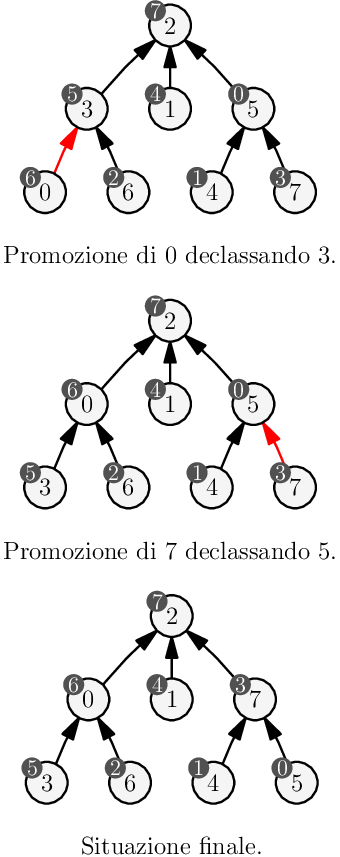
\includegraphics[scale=1]{asy_grattacieli/fig2.pdf}
\end{center}

In the \textbf{third sample testcase} the maximum sum of heights possible is
$54$,
and it can be obtained by choosing the following heights.

\begin{center}
\includegraphics[scale=1]{asy_grattacieli/fig3.pdf}
\end{center}
